Folgendes Entity Relationship (ER) Diagramm zeigt die Datenstruktur des Projektes:
\begin{figure}[H]
	\begin{center}
		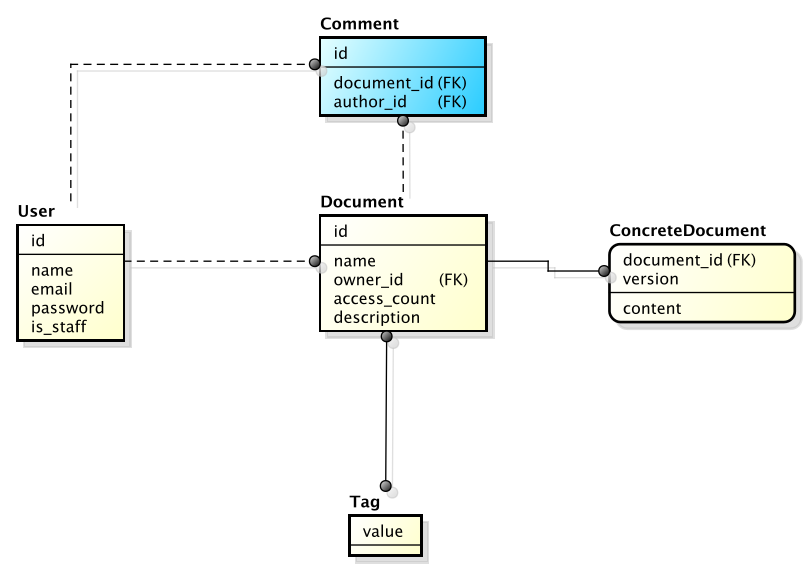
\includegraphics[width=\linewidth]{images/Datenstruktur.pdf}
		\caption{ER Diagramm}
	\end{center}
\end{figure}

\section{Weiterentwicklung}
Die Entwicklung und Versionierung der Datenbank erfolgt mit Migrationen.
Dabei handelt es sich um eine Funktionalit\"at des eingesetzten Frameworks, die Datenstruktur eines Projektes zu verwalten und entwickeln.

Hier ein Beispiel einer Migration, welche eine User Tabelle definiert.
\begin{lstlisting}[language={PHP}, caption=Beispiel eine Migration]
class CreateUsersTable extends Migration
{
  // Run the migrations.
  public function up()
  {
      Schema::create('users', function (Blueprint $table) {
          $table->increments('id');
          $table->string('name');
          $table->string('email')->unique();
          $table->string('password', 60);
          $table->rememberToken();
          $table->timestamps();
      });
  }

  // Reverse the migrations.
  public function down()
  {
      Schema::drop('users');
  }
}
\end{lstlisting}

Eine Migration wird erstellt mittels \texttt{php artisan create:migration [name]} und ist dann unter dem Ordner \texttt{database/migrations} mit allen bisherigen Migrationen zu finden und zu editieren.
Um dann die Datenbank zu migrieren (Datenstruktur in der Datenbank erstellen, nicht zu verwechseln mit dem erstellen Migrationsscript) wird der Befehl \texttt{php artisan migrate} ausgef\"uhrt.

Eine genauere Dokumentation zu Migrationen in Laravel ist in der offiziellen Dokumentation von Laravel unter \url{https://laravel.com/docs/5.2/migrations} zu finden.
